\chapter{Simulation Set-up}
\label{wasenmoos_model}
This chapter discusses the translation of a part of the study area, as described in the previous chapter, into a numerical description in the form of GW and SW models, the setting up of the coupling scheme, and the application of the GWSWEX model to the same. The following chapter visualizes the results of this simulation and draws plausible conclusions from the same.
\\ \\
Modflow 6 (refer \ref{mf6}) is used to simulate the GW processes, D-Flow FM (refer \ref{delft}) is used to simulate the SW processes, and GWSWEX (refer \ref{GWSWEX}) is used as the precursor interface model, along with the coupling scheme (refer \ref{couping_scheme}) to couple these two models and thus effectively the processes that they represent. The GWSWEX python module (refer \ref{GWSWEXpy}) is used to set up the simulation.   

\section{Temporal Discretization}
The simulation period starts on 01.05.2020 at 00:00:00 and ends on 01.06.2020 at 00:00:00. Each local simulation period lasts for 3600 seconds i.e. the models exchange information every \unit[3600]{s} via the coupling scheme.
The number of internal time-steps per local simulation period, however, is controlled automatically by the GWSWEX module based on the precipitation intensity. Here, it is limited to 1 time-step when the precipitation intensity is \unit[0]{mm/h} and increased to 15 time-steps when precipitation intensity exceeds \unit[1]{mm/h}.

\section{Spatial Discretization}
Since the nature of coupling is explicit and since the GWSWEX model is based on the assumption that the spatial discretization of the GW and SW models are exactly similar, the study uses the same unstructured grid layout for both GW and SW models. As observed in Figure \ref{fig:grid_qgis}, this study models a portion of the study area in the interest of keeping the runtimes low, to enable swift testing and debugging, both, of the coupling scheme and the GWSWEX model. Figure \ref{fig:grid_bed_levels} shows the surface level elevation of the model grid. The elevations have been obtained by combining a \unit[1]{m} raster with individual stream-bed measurements taken along the dewatering stream.
\\ \\
The grid is bounded on the east by the ridge formation, the north boundary is bordered by a stream running along it, the boundary on the west runs perpendicular to the observed GW isolines and is relatively flat, and the southern boundary is runs along a relatively flat area. Thus they are regarded as no-flow boundaries.
The discretization is rather coarse overall but finer at the stream.
\\ \\
The total number of elements in the model grid is 2948, spanning over an area of around \unit[65940]{$m^2$}.

\begin{figure}[h!]
    \centering
    \includegraphics[width=\linewidth]{PICTURES/models_ini/grid_qgis.png}
    \caption{Model Grid. Elements coloured blue represent elements that are a part of the stream and those in red signify active boundaries.}
    \label{fig:grid_qgis}
\end{figure}

\begin{figure}[h!]
    \centering
    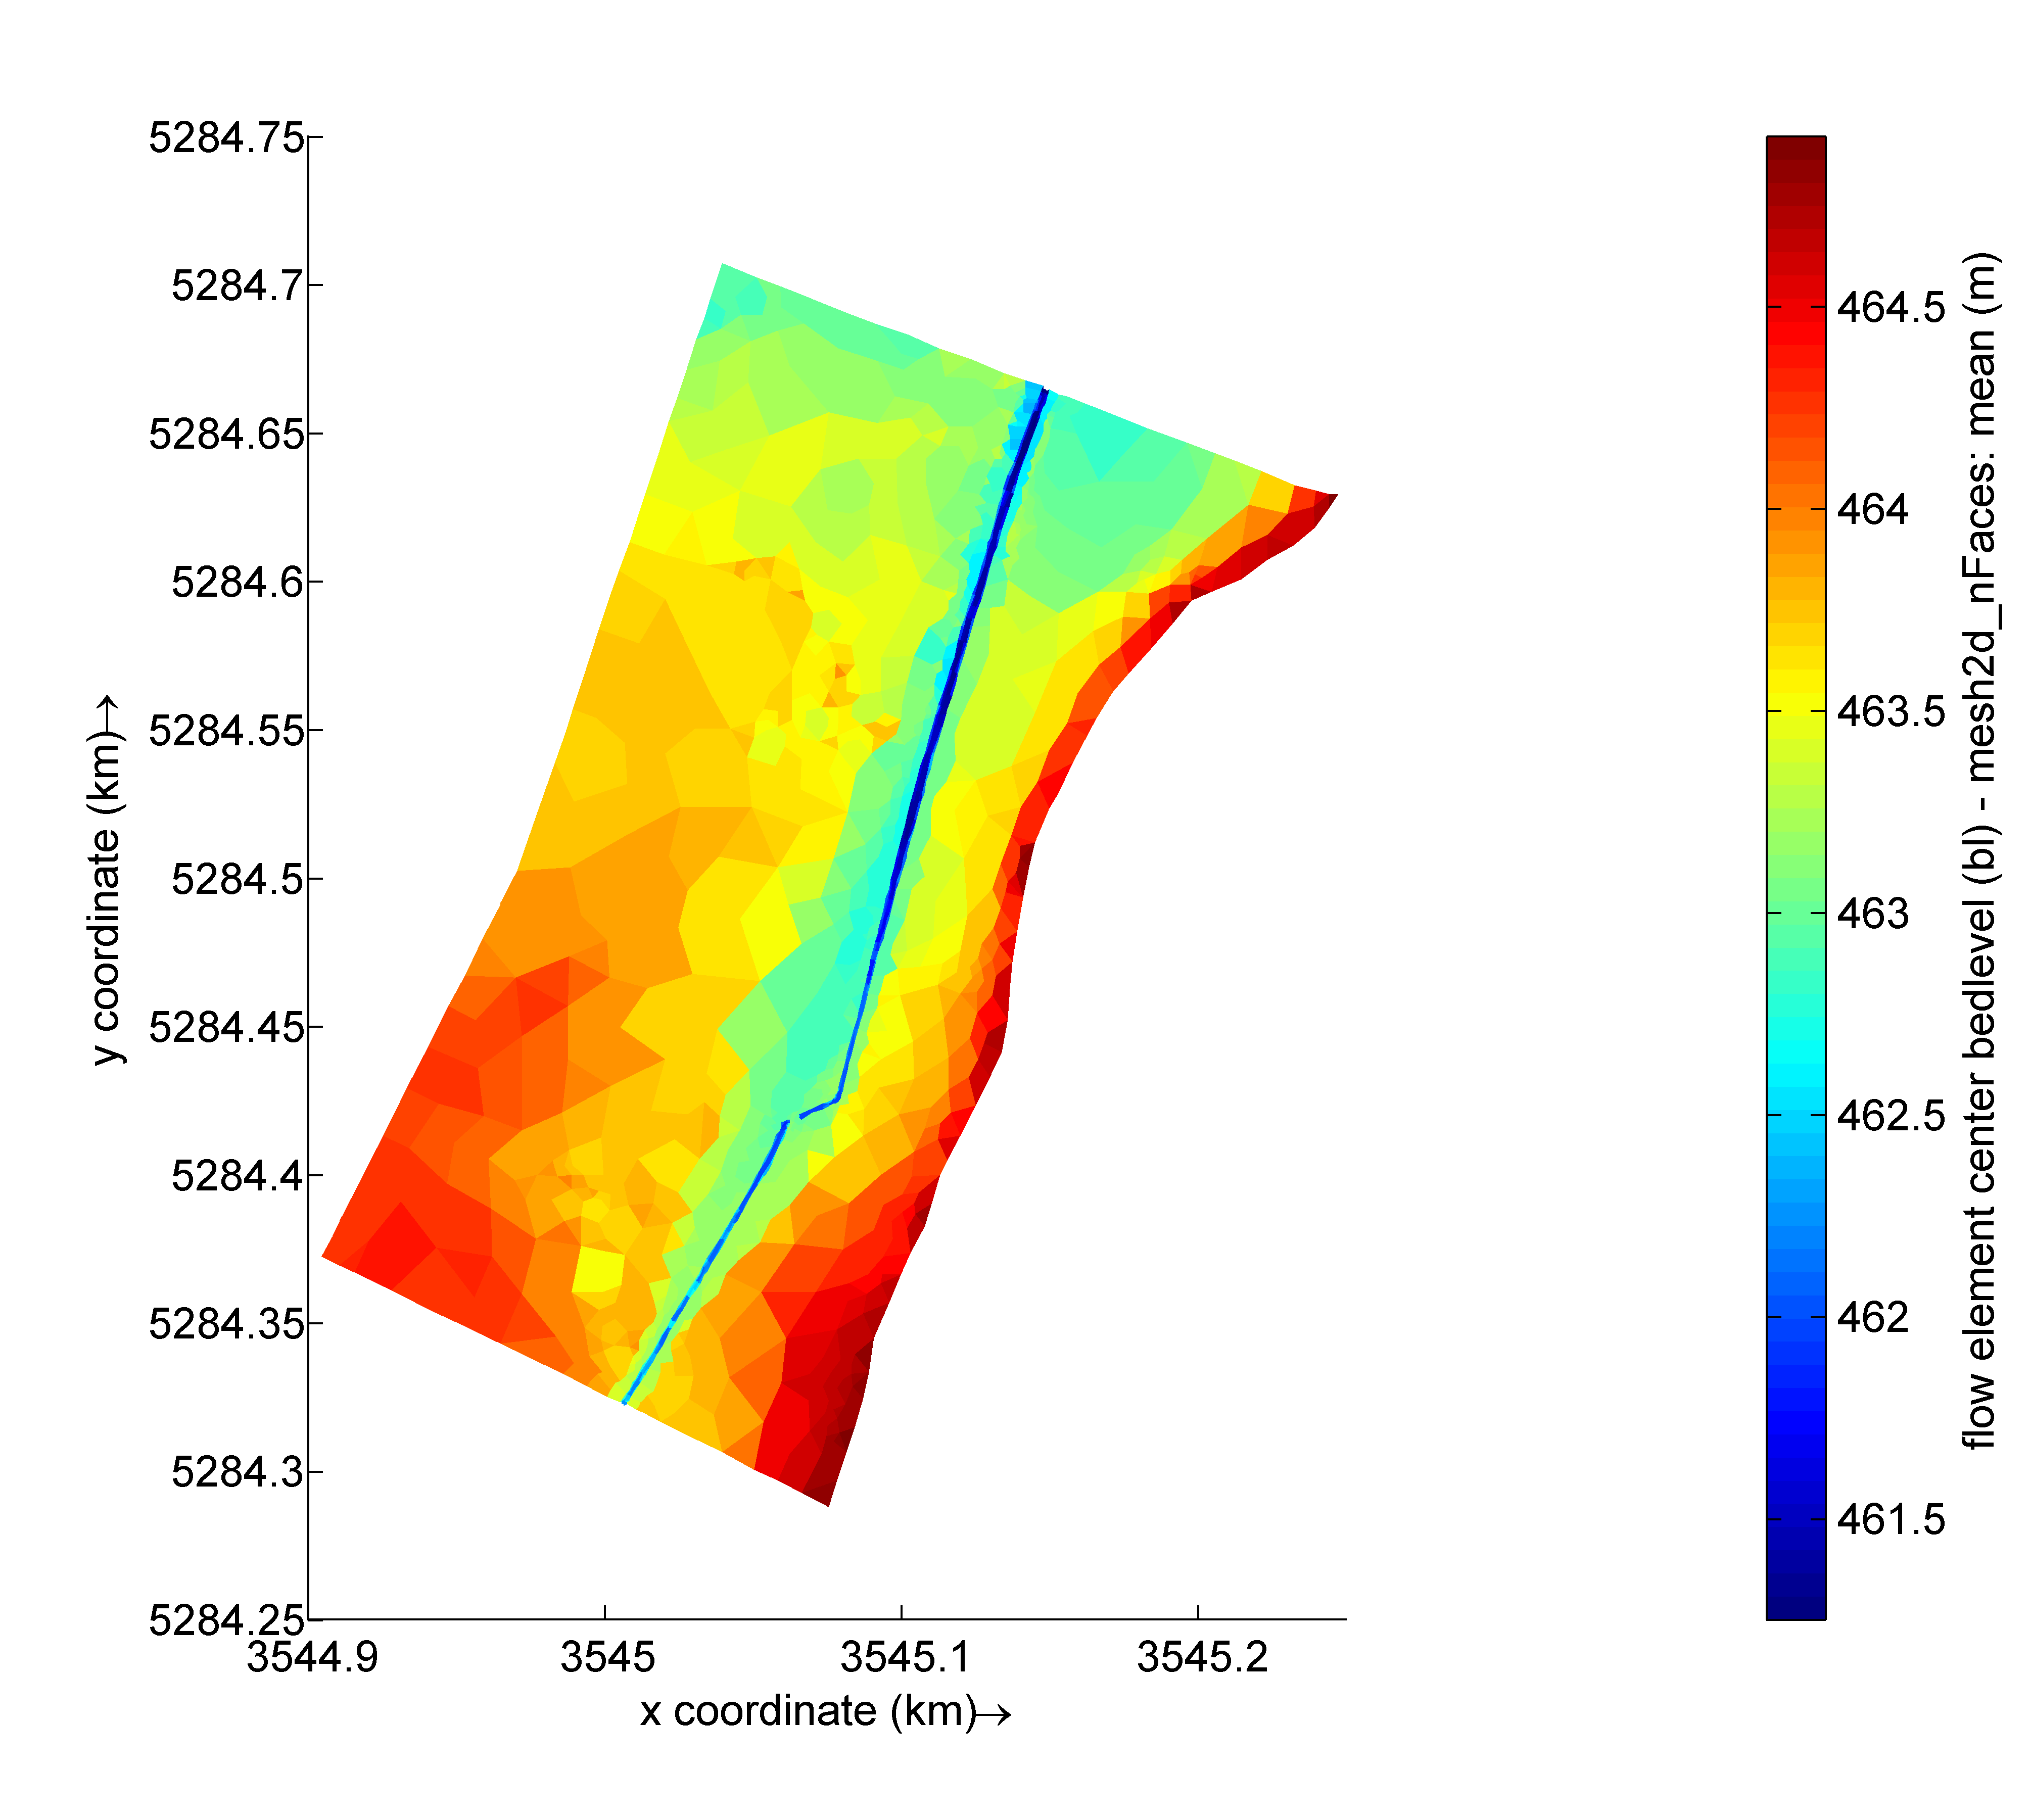
\includegraphics[scale=0.8]{PICTURES/models_ini/bed_levels.png}
    \caption{Surface Elevation of the Model Grid.}
    \label{fig:grid_bed_levels}
\end{figure}

\section{Model Parameters and Regular Inputs}
This section mentions the inputs and parameters used for the models and briefly discusses the rationale for using the same, if necessary.

\subsection{GWSWEX}
Refer \ref{GWSWEX_input}.
\begin{itemize}
    \item precipitation influxes are obtained from the German Weather Service (DWD) for the station \textit{Weingarten, Ravensburg}.
    \item evapotranspiration outfluxes are obtained from previous calculations in the parent study.
    \item n is linked to the specific yield of the unconfined aquifer set in the GW model.
    \item n\textunderscore gw is linked to the specific storage of the unconfined aquifer set in the GW model,
    \item m = 0.3, decided as an initial guess.
    \item k is linked to the hydraulic conductivity of the unconfined aquifer set in the GW model.
    \item $\alpha$ = 0.15, decided as an initial guess.
    \item $\beta$ = 0.7, decided as an initial guess.
    \item $SW_th$ = 0.05, decided as an initial guess based on the ET fluxes and the local simulation time period.
\end{itemize}

\subsection{Modflow 6}
The GW model is set up on Modflow 6 (refer \ref{mf6}) in accordance with the hydrogeological properties as illustrated in \ref{fig:wasenmoosCS}. The top of the model corresponds to the ground surface elevation. The bottom of the unconfined aquifer is set to the lowest elevation of the stream. It is to be assessed if this is an adequately realistic representation of reality. Figure \ref{fig:aq0_thickness} shows the thickness of the unconfined aquifer over the model grid. The aquitard layer and the confined layer are assumed to be uniformly thick, each bearing a thickness of \unit[1]{m} and \unit[10]{m} respectively.

\begin{figure}[h!]
    \centering
    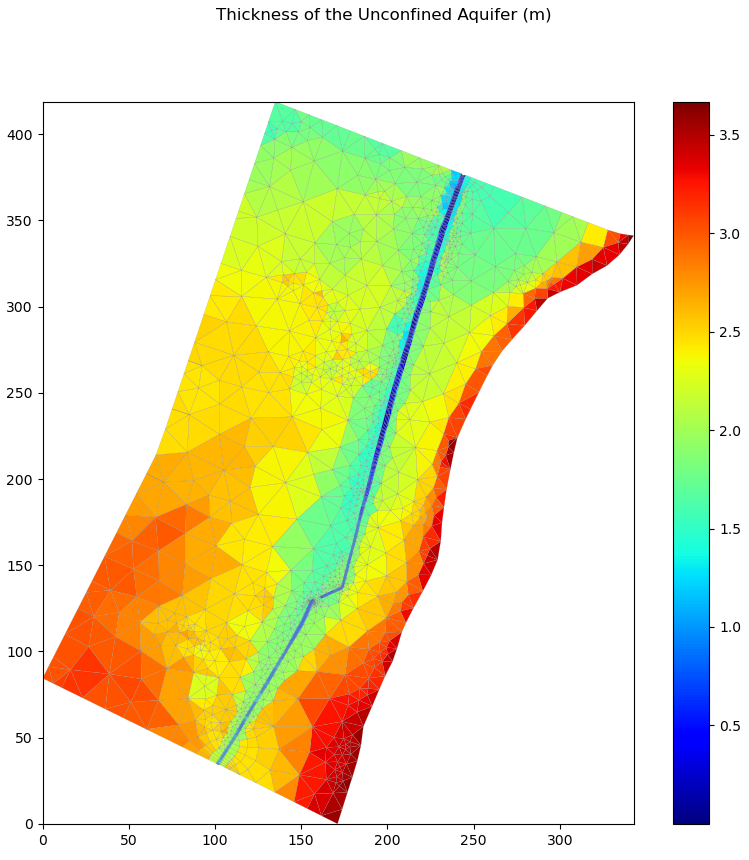
\includegraphics[scale=0.42]{PICTURES/models_ini/aq0_thickness.png}
    \caption{Thickness of the Unconfined Aquifer (m).}
    \label{fig:aq0_thickness}
\end{figure}

The assumptions for hydraulic conductivities ($K$), specific yields ($S_y$), and specific storages ($S_s$) for the three layers, based on peer-reviewed literature are as follows \cite{Rezanezhad2016} \cite{Lennartz} \cite{Lu2015} \cite{Shestakov2002} \cite{Schlotzhauer1999}:
\begin{table}[h!]
\caption{Assumed hydrogeological properties}
\label{tab:hydrogeoIP}
\centering
\begin{tabular}{llll}
\hline\noalign{\smallskip}
aquifer & $K$ & $S_y$ & $S_s$  \\
\noalign{\smallskip}\hline\noalign{\smallskip}
unconfined aquifer & \SI{5e-4}{\meter\per\second} & 0.4 & \SI{6e-3}{\per\meter} \\
clay aquitard & \SI{3e-9}{\meter\per\second} & 0.15 & \SI{1e-3}{\per\meter} \\
confined aquifer & \SI{1e-4}{\meter\per\second} & 0.15 & \SI{2e-5}{\per\meter} \\
\noalign{\smallskip}\hline
\end{tabular}
\end{table}

\subsection{D-Flow FM}
The setup of the SW model is rather quite simple, stemming partially from the fact that the SW processes and storages are not very dominant in this study in comparison to the GW storages and processes, and partially from the undemanding nature of required model parameters to set up the D-Flow FM model.
\\
The Manning's coefficient is set to 0.23 over the model domain and to 0.05 at the stream.

\section{Initial Conditions}

\subsection{GWSWEX}
The initial GW and SW levels are read from the GW and SW models respectively. Initial SM levels are set to 80\% saturation of the ePV. It is to be assessed whether this is a adequately realistic assumption.
\begin{figure}[!h]
\minipage{0.5\textwidth}
  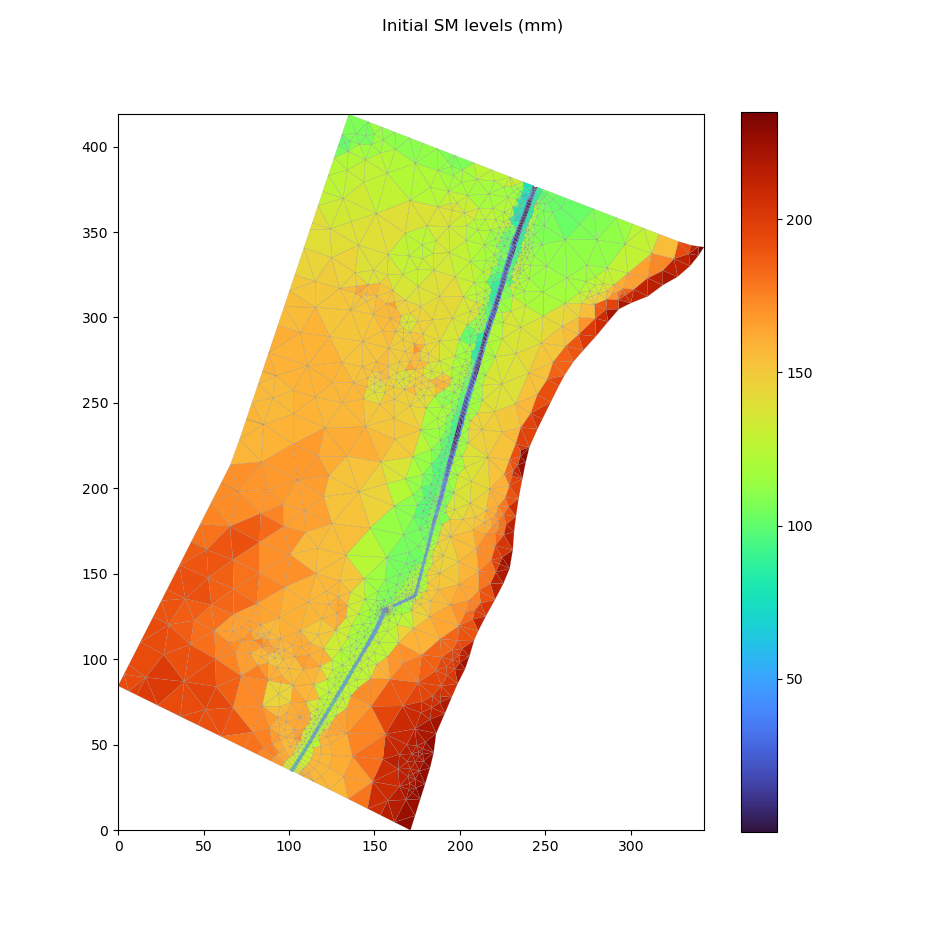
\includegraphics[width=\linewidth]{PICTURES/models_ini/sm_ini}
\endminipage\hfill
\minipage{0.5\textwidth}
  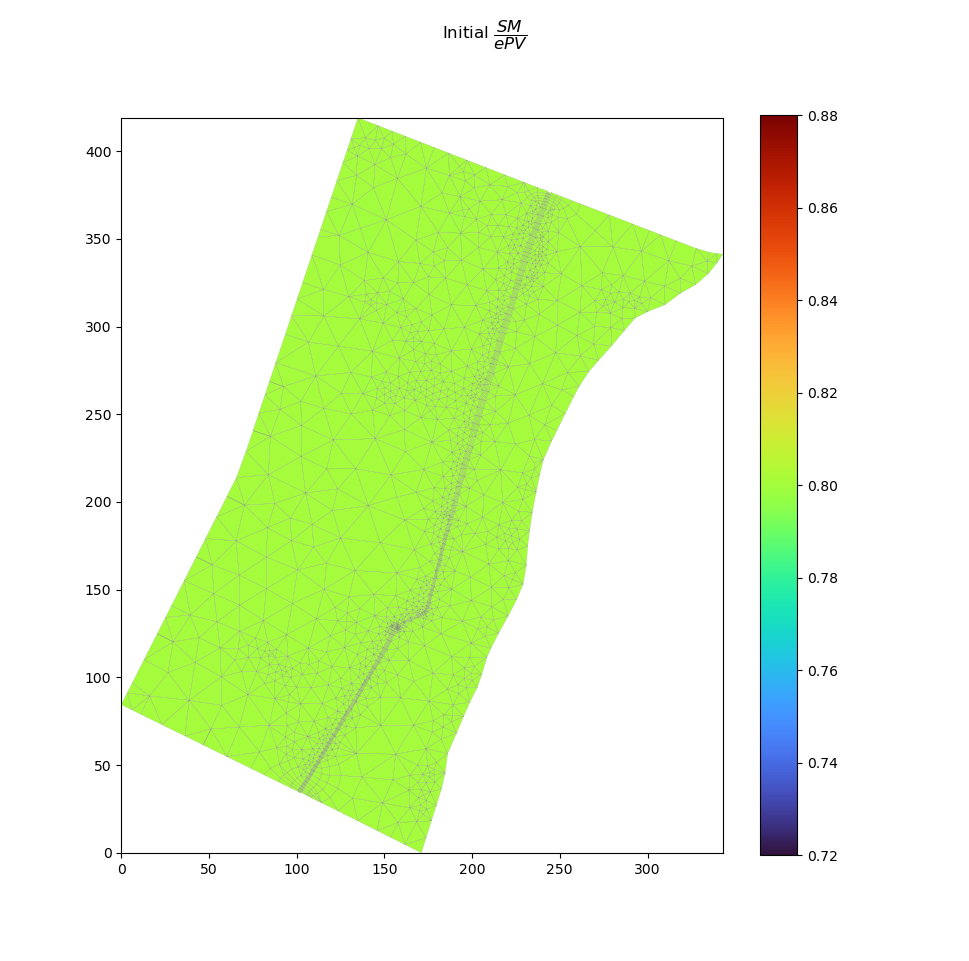
\includegraphics[width=\linewidth]{PICTURES/models_ini/sm_ini_ratio}
\endminipage\hfill
\caption{Initial soil moisture: left - absolute levels (mm); right - relative saturation.}\label{fig:sm_ini}
\end{figure}

\subsection{Modflow 6}
The starting heads for the unconfined aquifer was set to 80\% saturation. This corresponds to the GW level observed in observation point P-7 (refer Figure \ref{fig:obs_pts} for location). This way, the heads would correspond to the trends of the surface elevation. The starting heads for the aquitard and the confined aquifer are set at \unit[0.1]{m} above the model top elevation. It is to be assessed how these assumptions hold true.

\begin{figure}[!h]
\minipage{0.32\textwidth}
  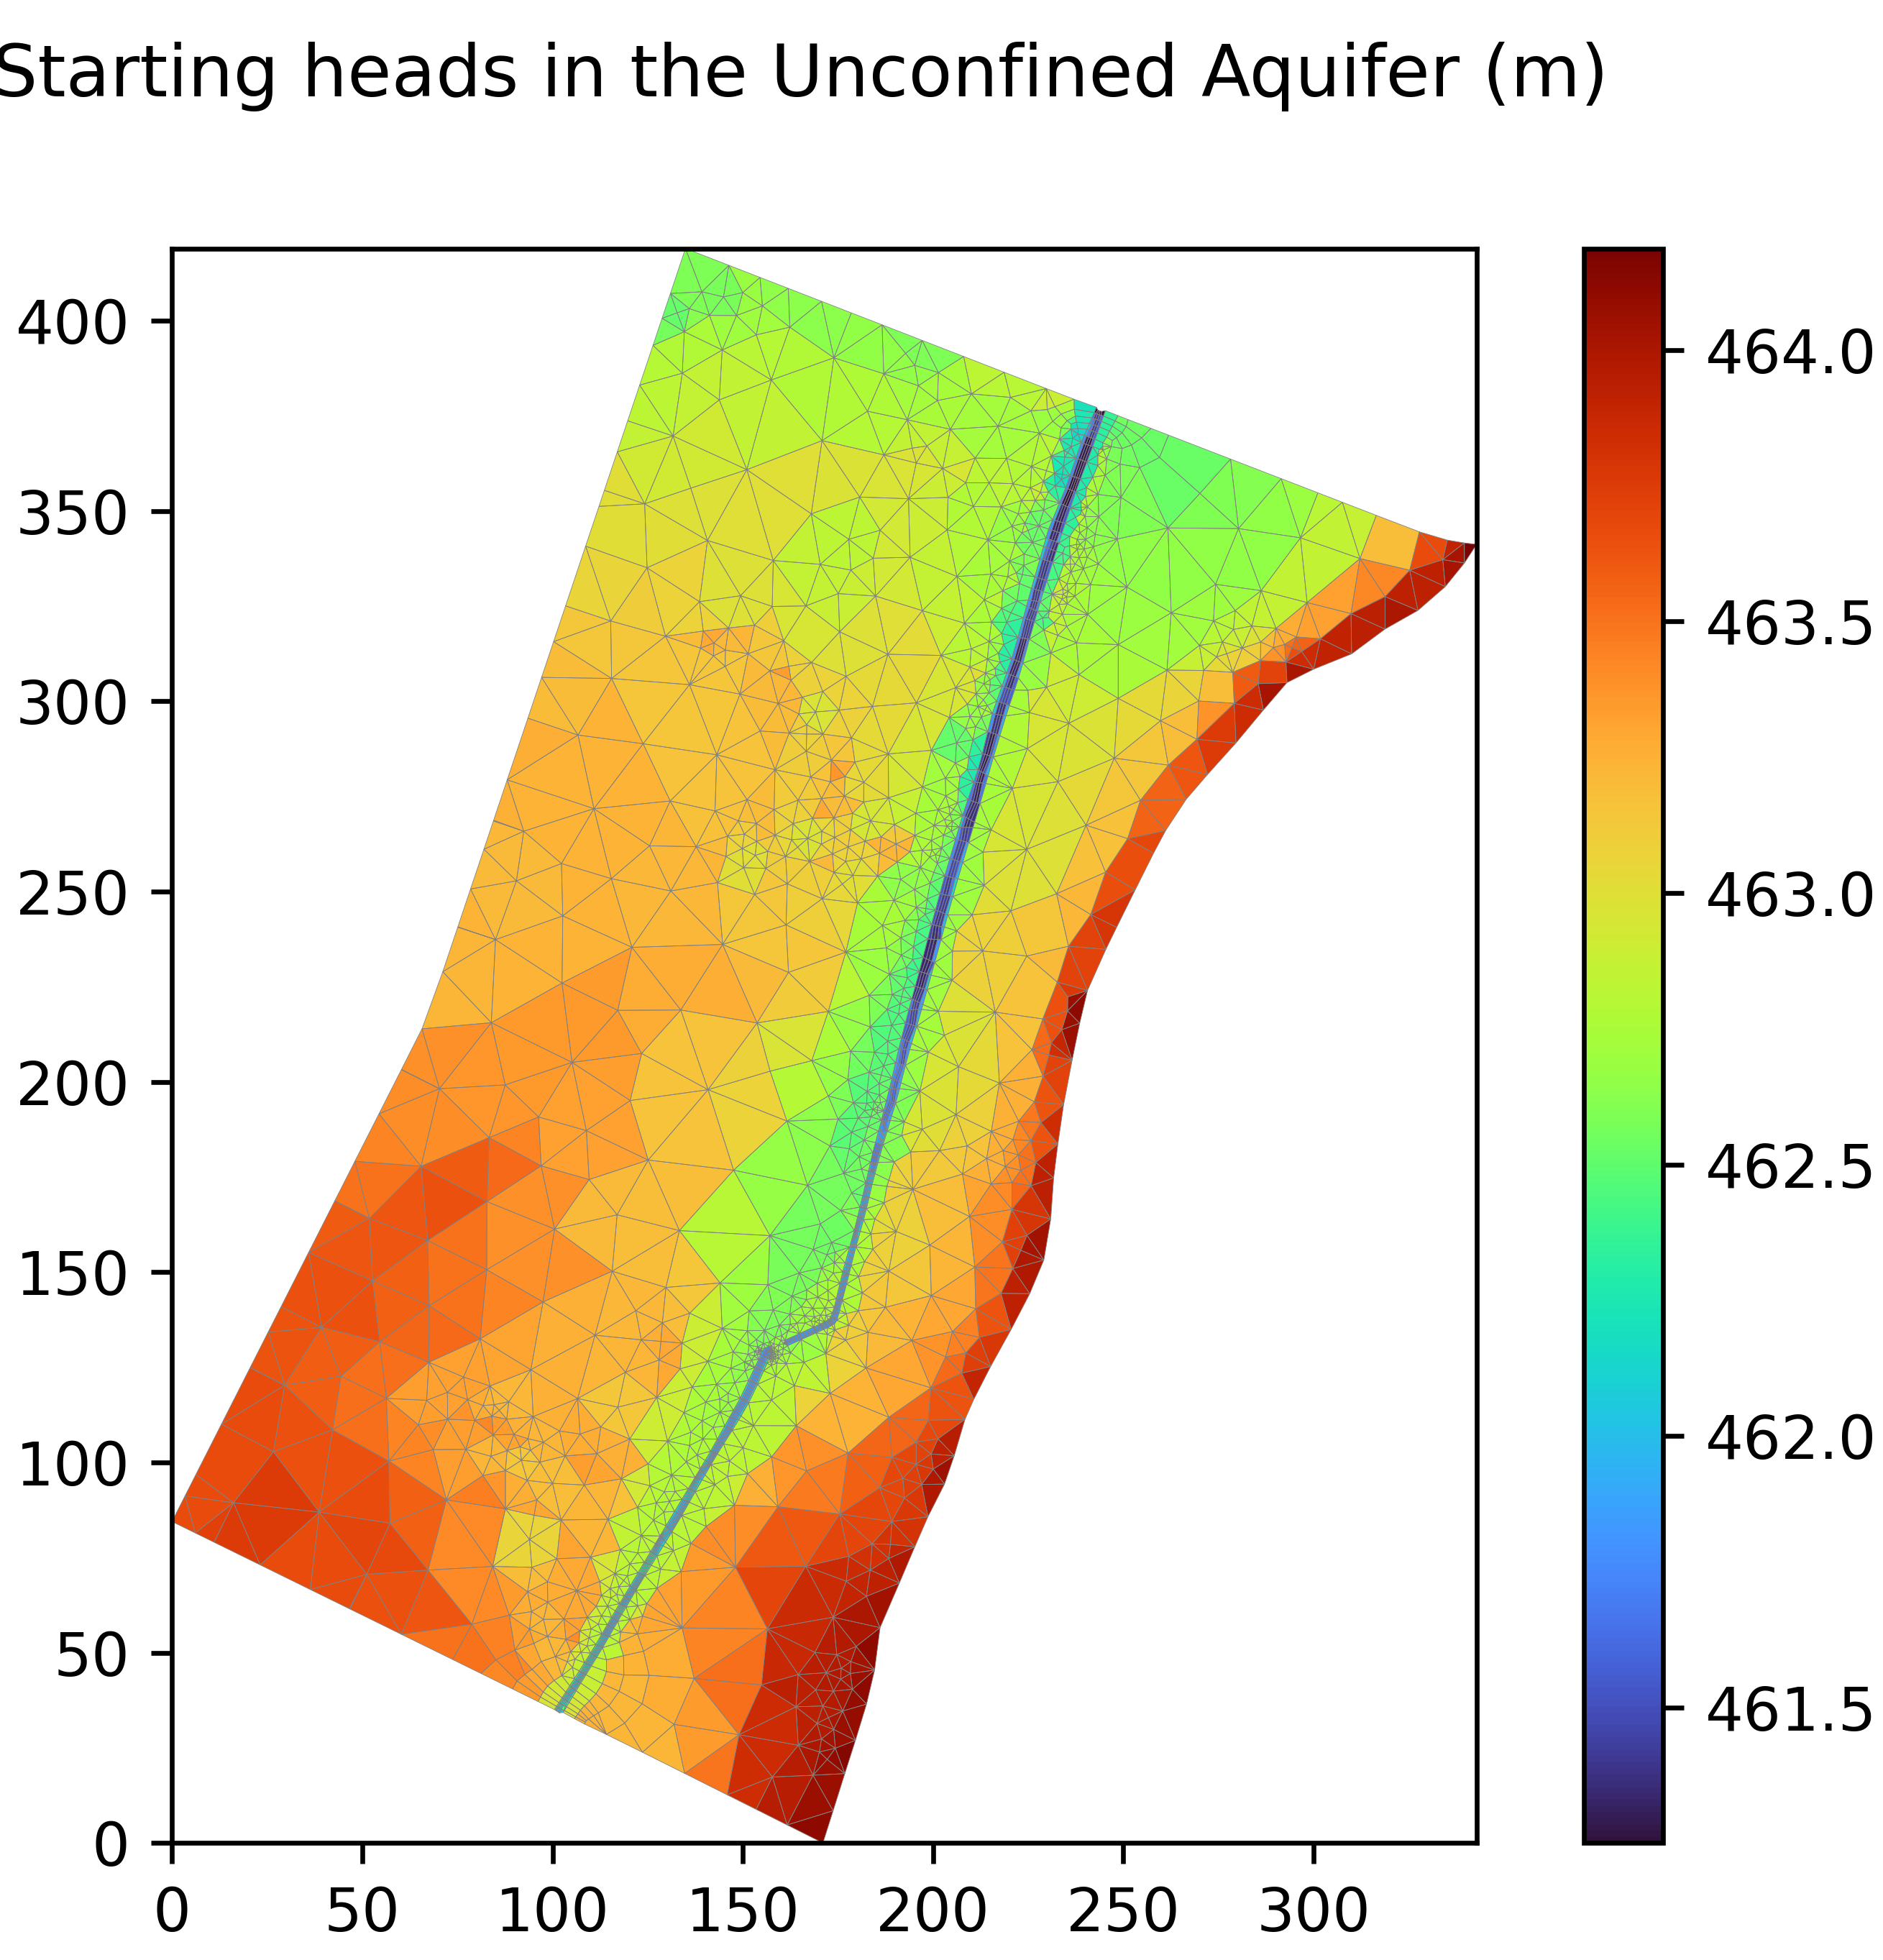
\includegraphics[width=\linewidth]{PICTURES/models_ini/strt_aq0}
\endminipage\hfill
\minipage{0.32\textwidth}
  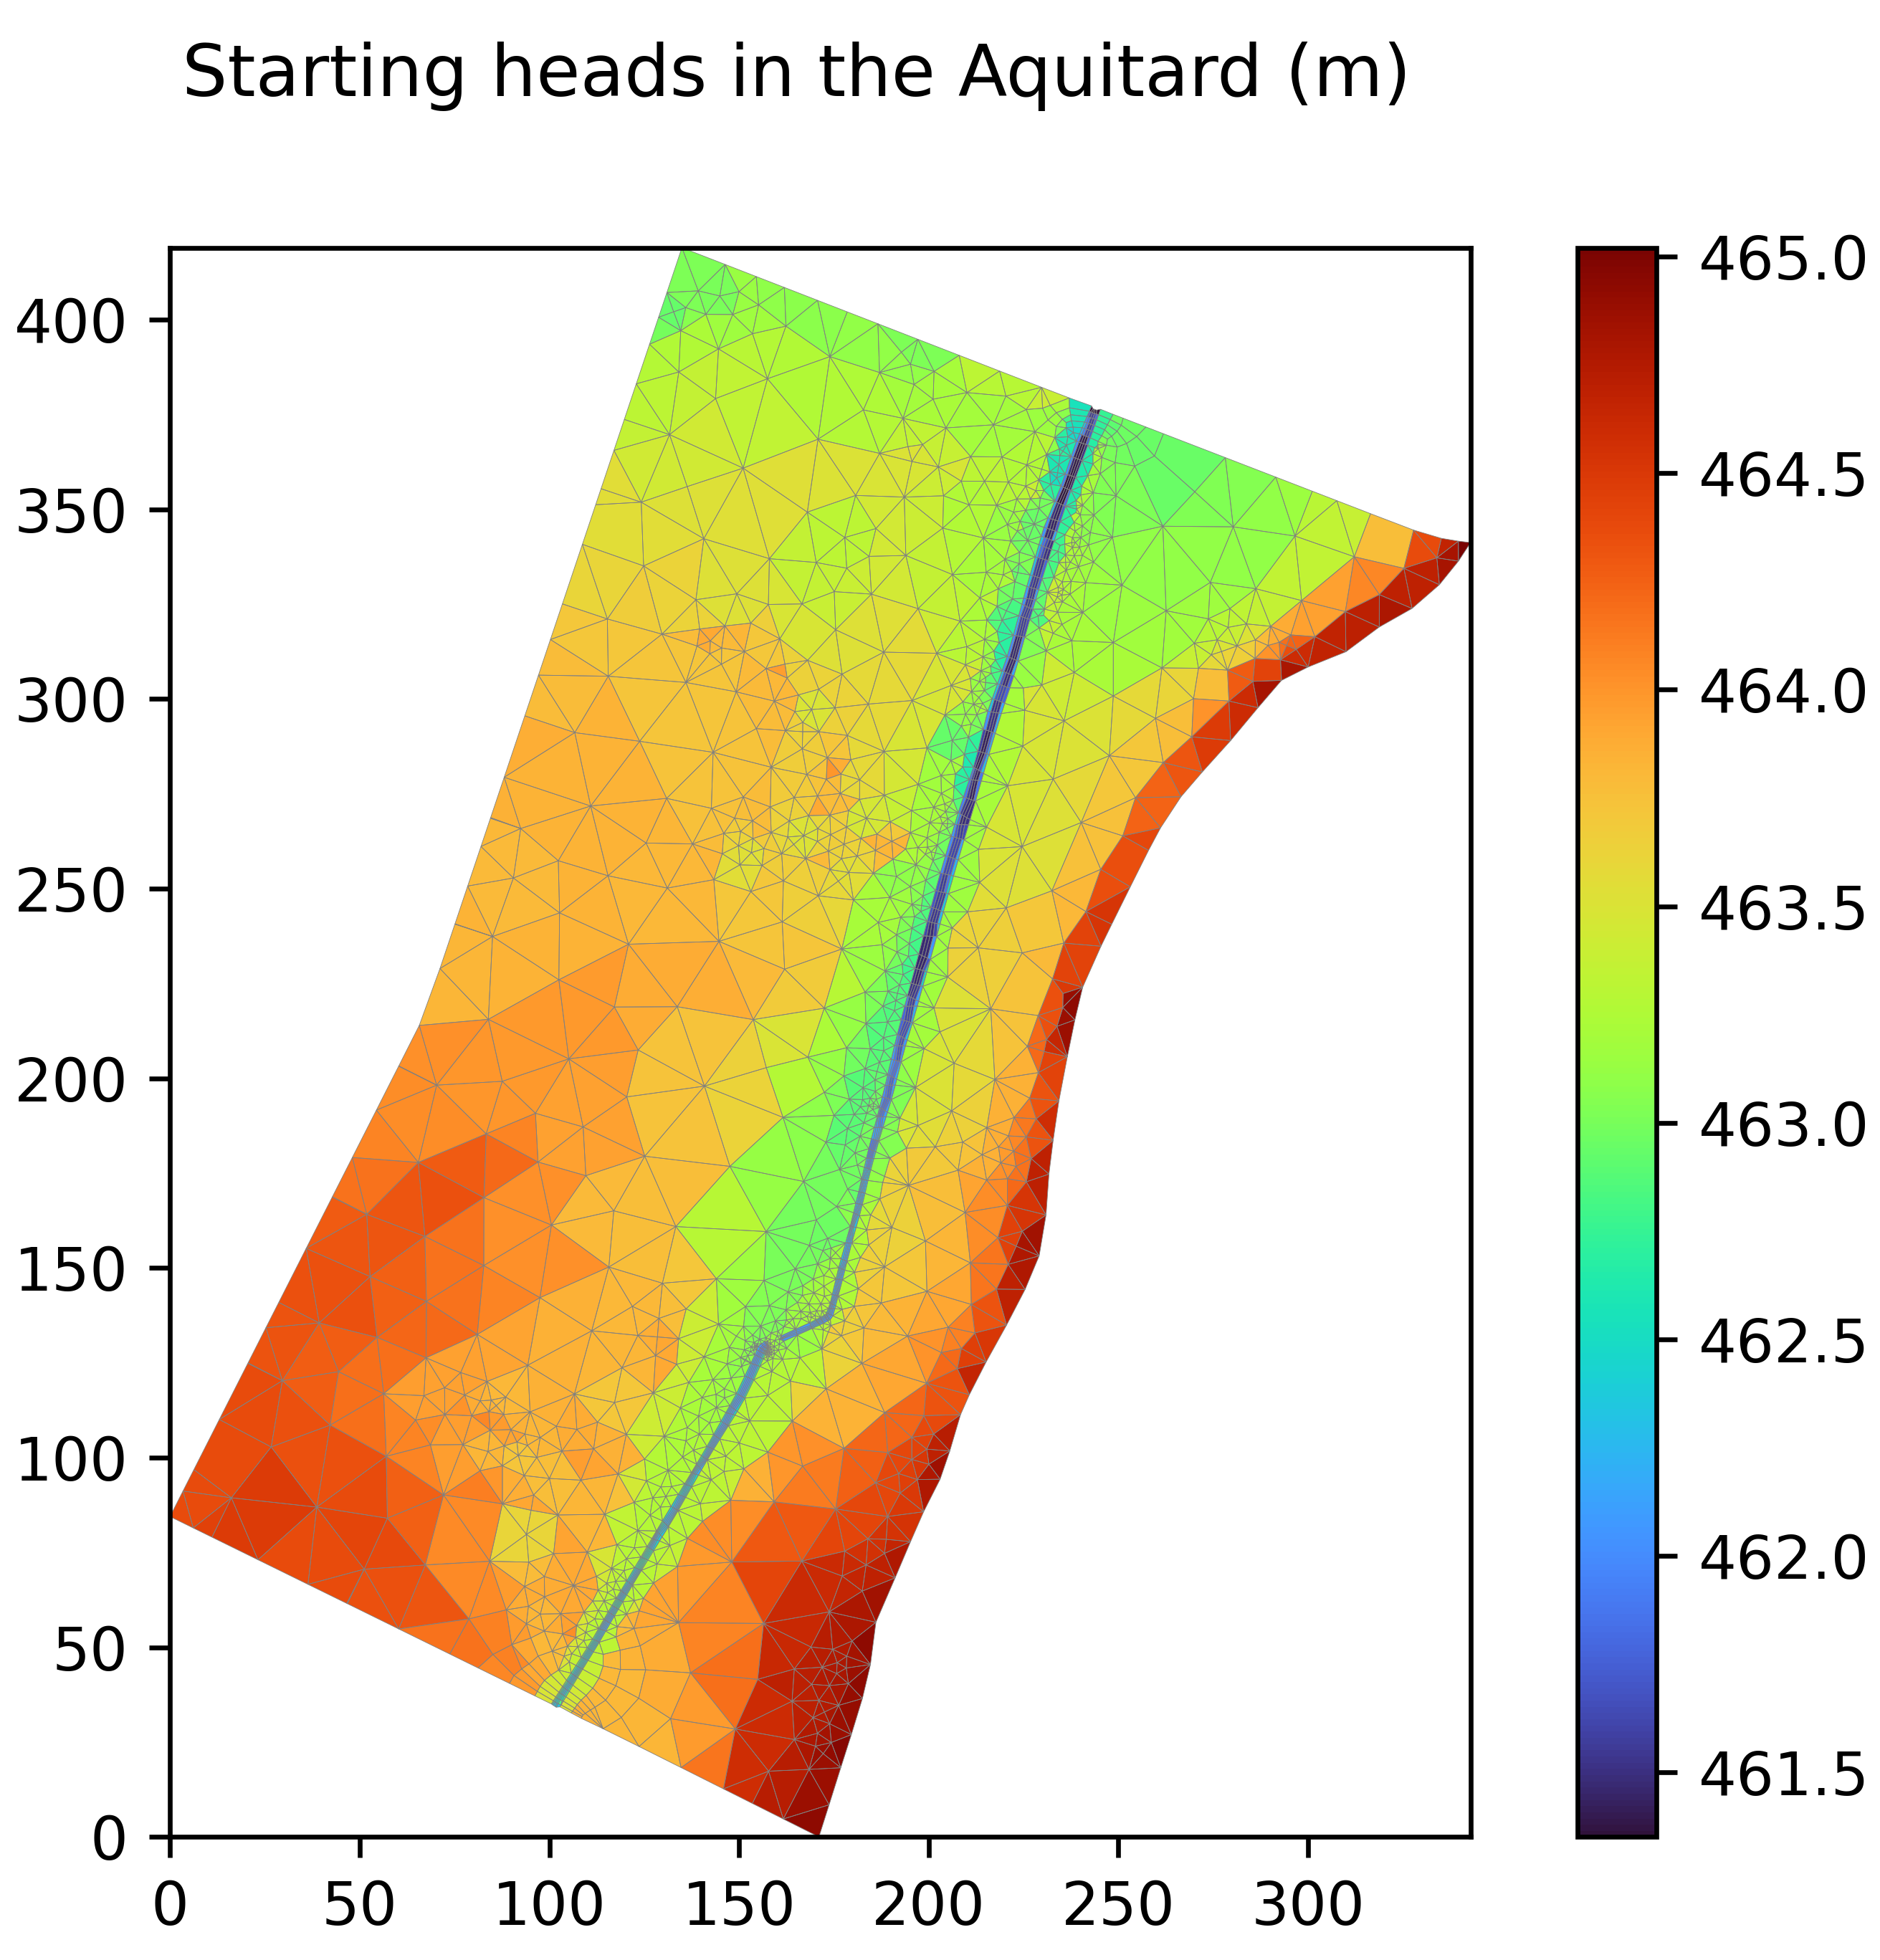
\includegraphics[width=\linewidth]{PICTURES/models_ini/strt_aq1}
\endminipage\hfill
\minipage{0.32\textwidth}
  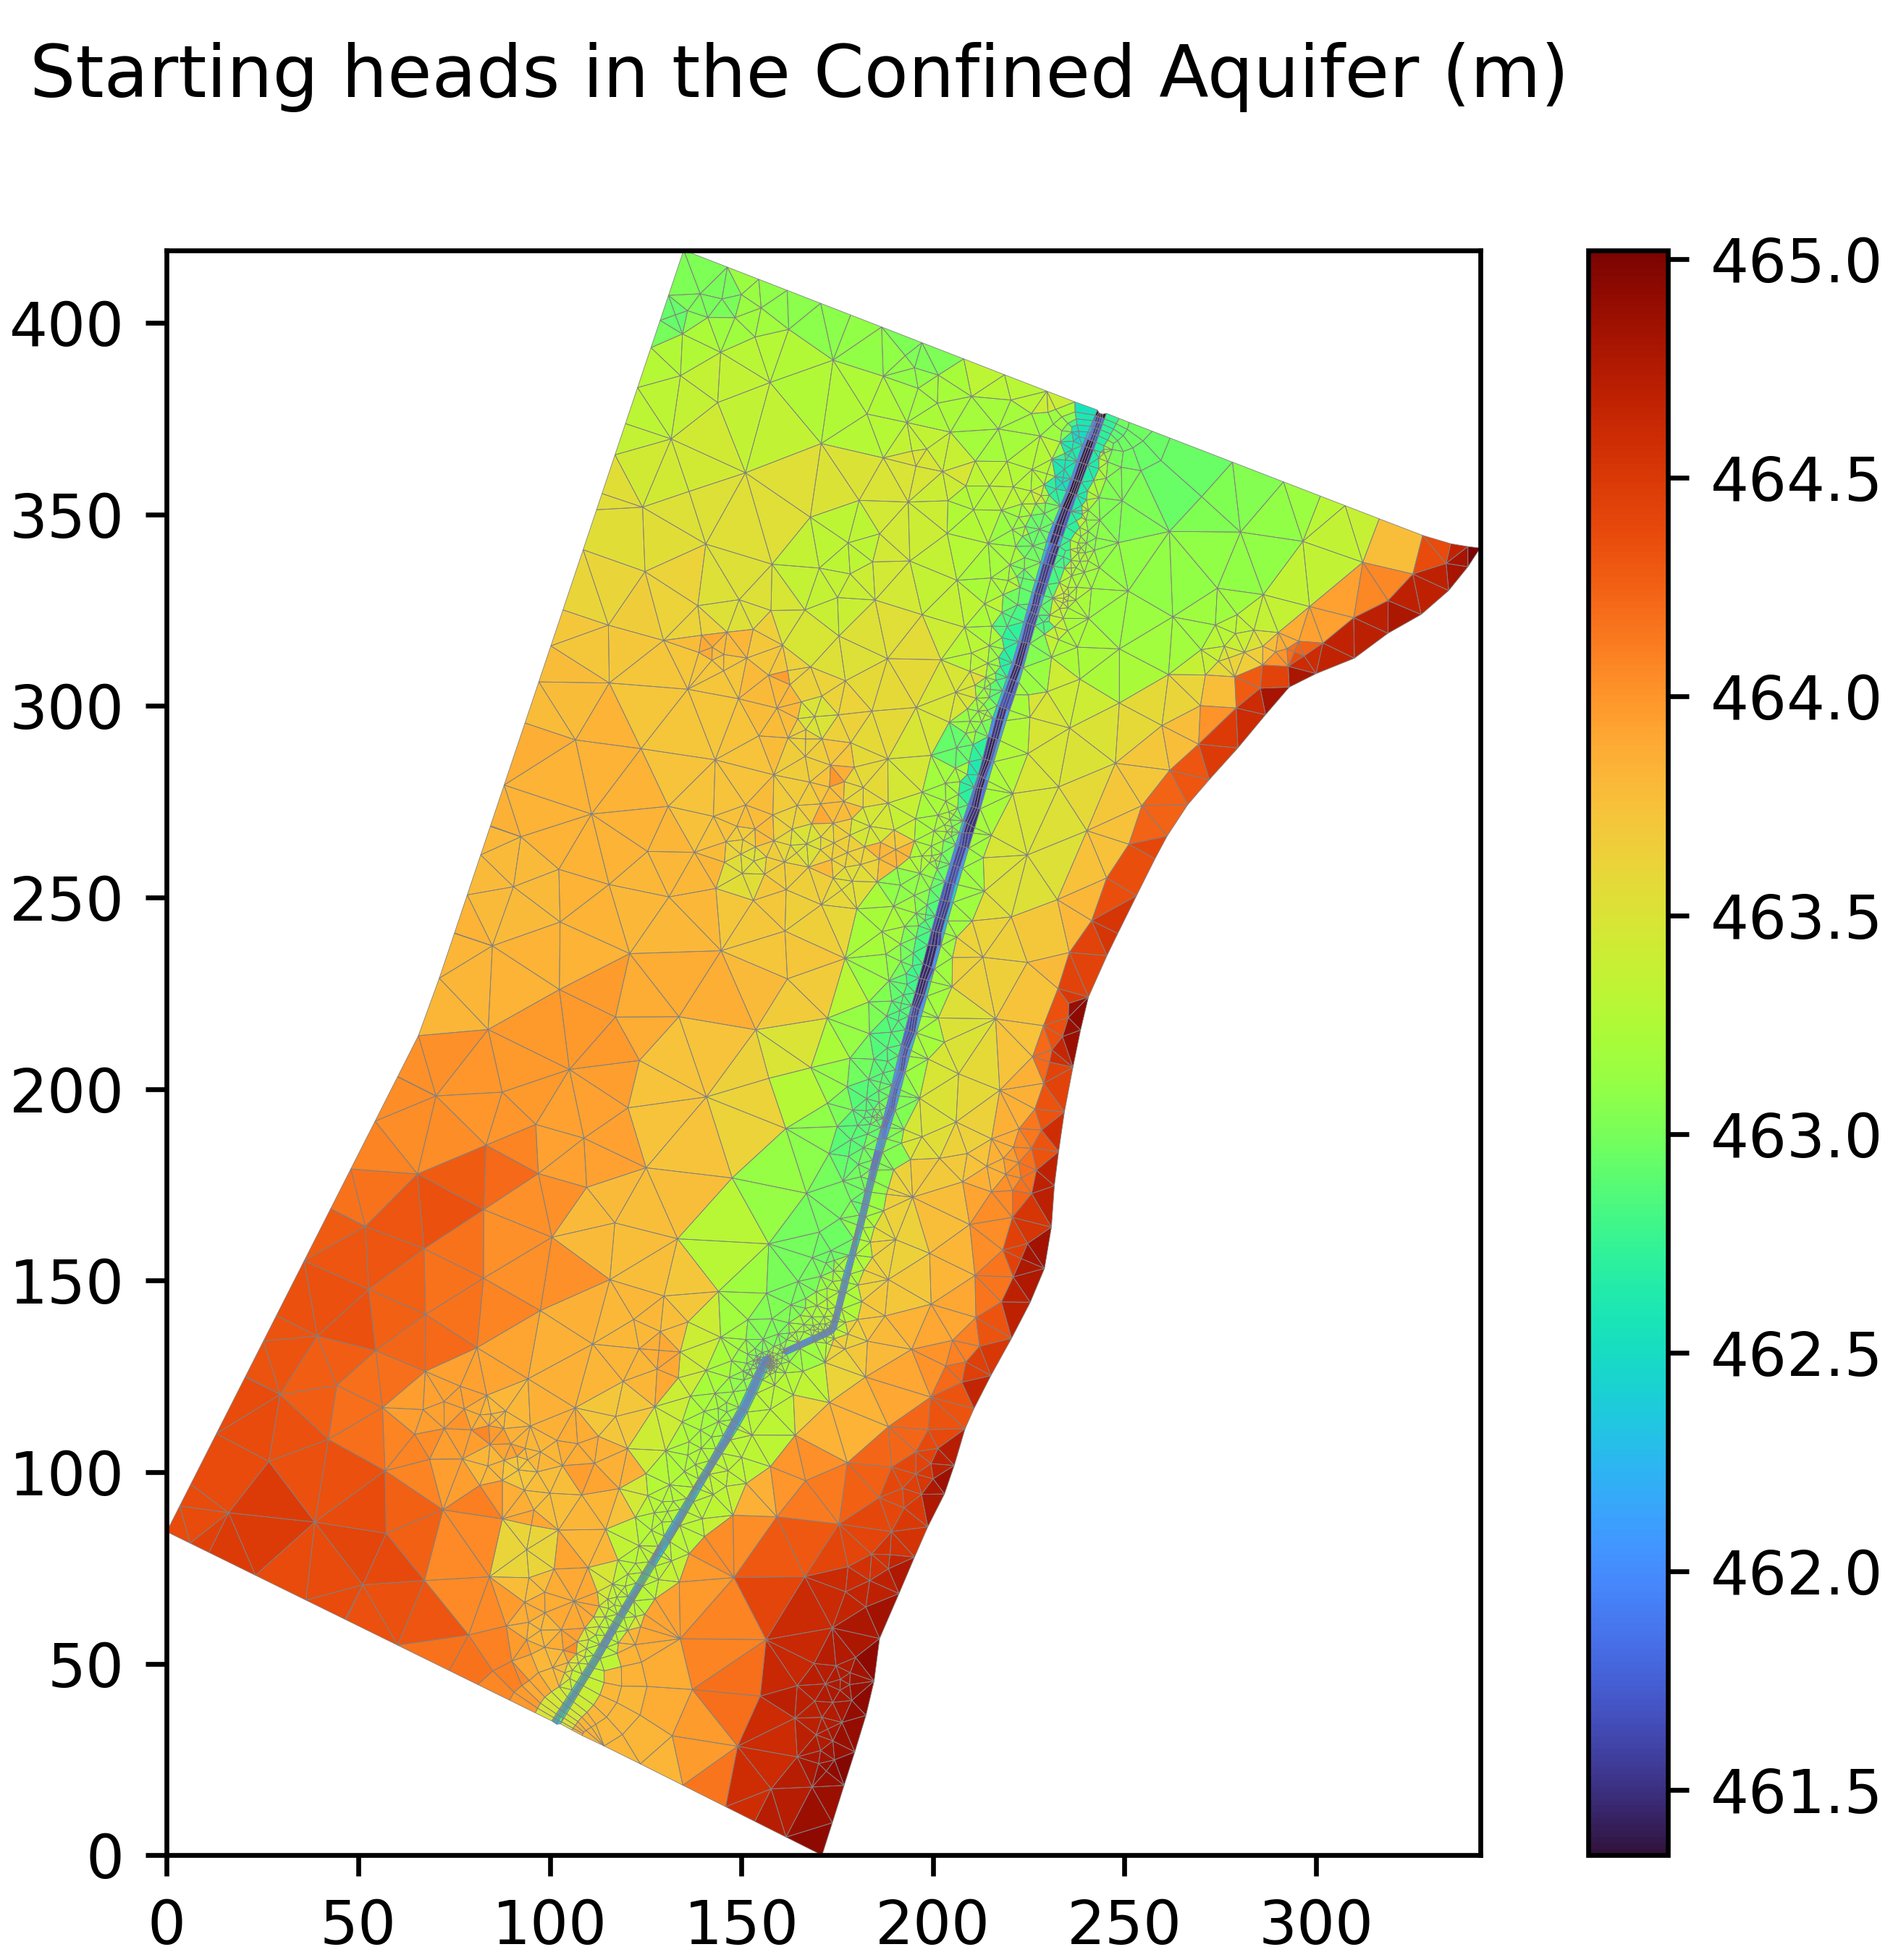
\includegraphics[width=\linewidth]{PICTURES/models_ini/strt_aq2}
\endminipage
\caption{Starting heads in the GW Model.}\label{fig:mf6_ic_strt}
\end{figure}

\subsection{D-Flow FM}
Initial water levels just adequate for all model cells to be considered wet are prescribed as starting water levels in the SW model. This is expected to correspond to reality as the system is not SW dominant and precipitation influx right before the start of the simulation period is sparse.

\begin{figure}[h!]
    \centering
    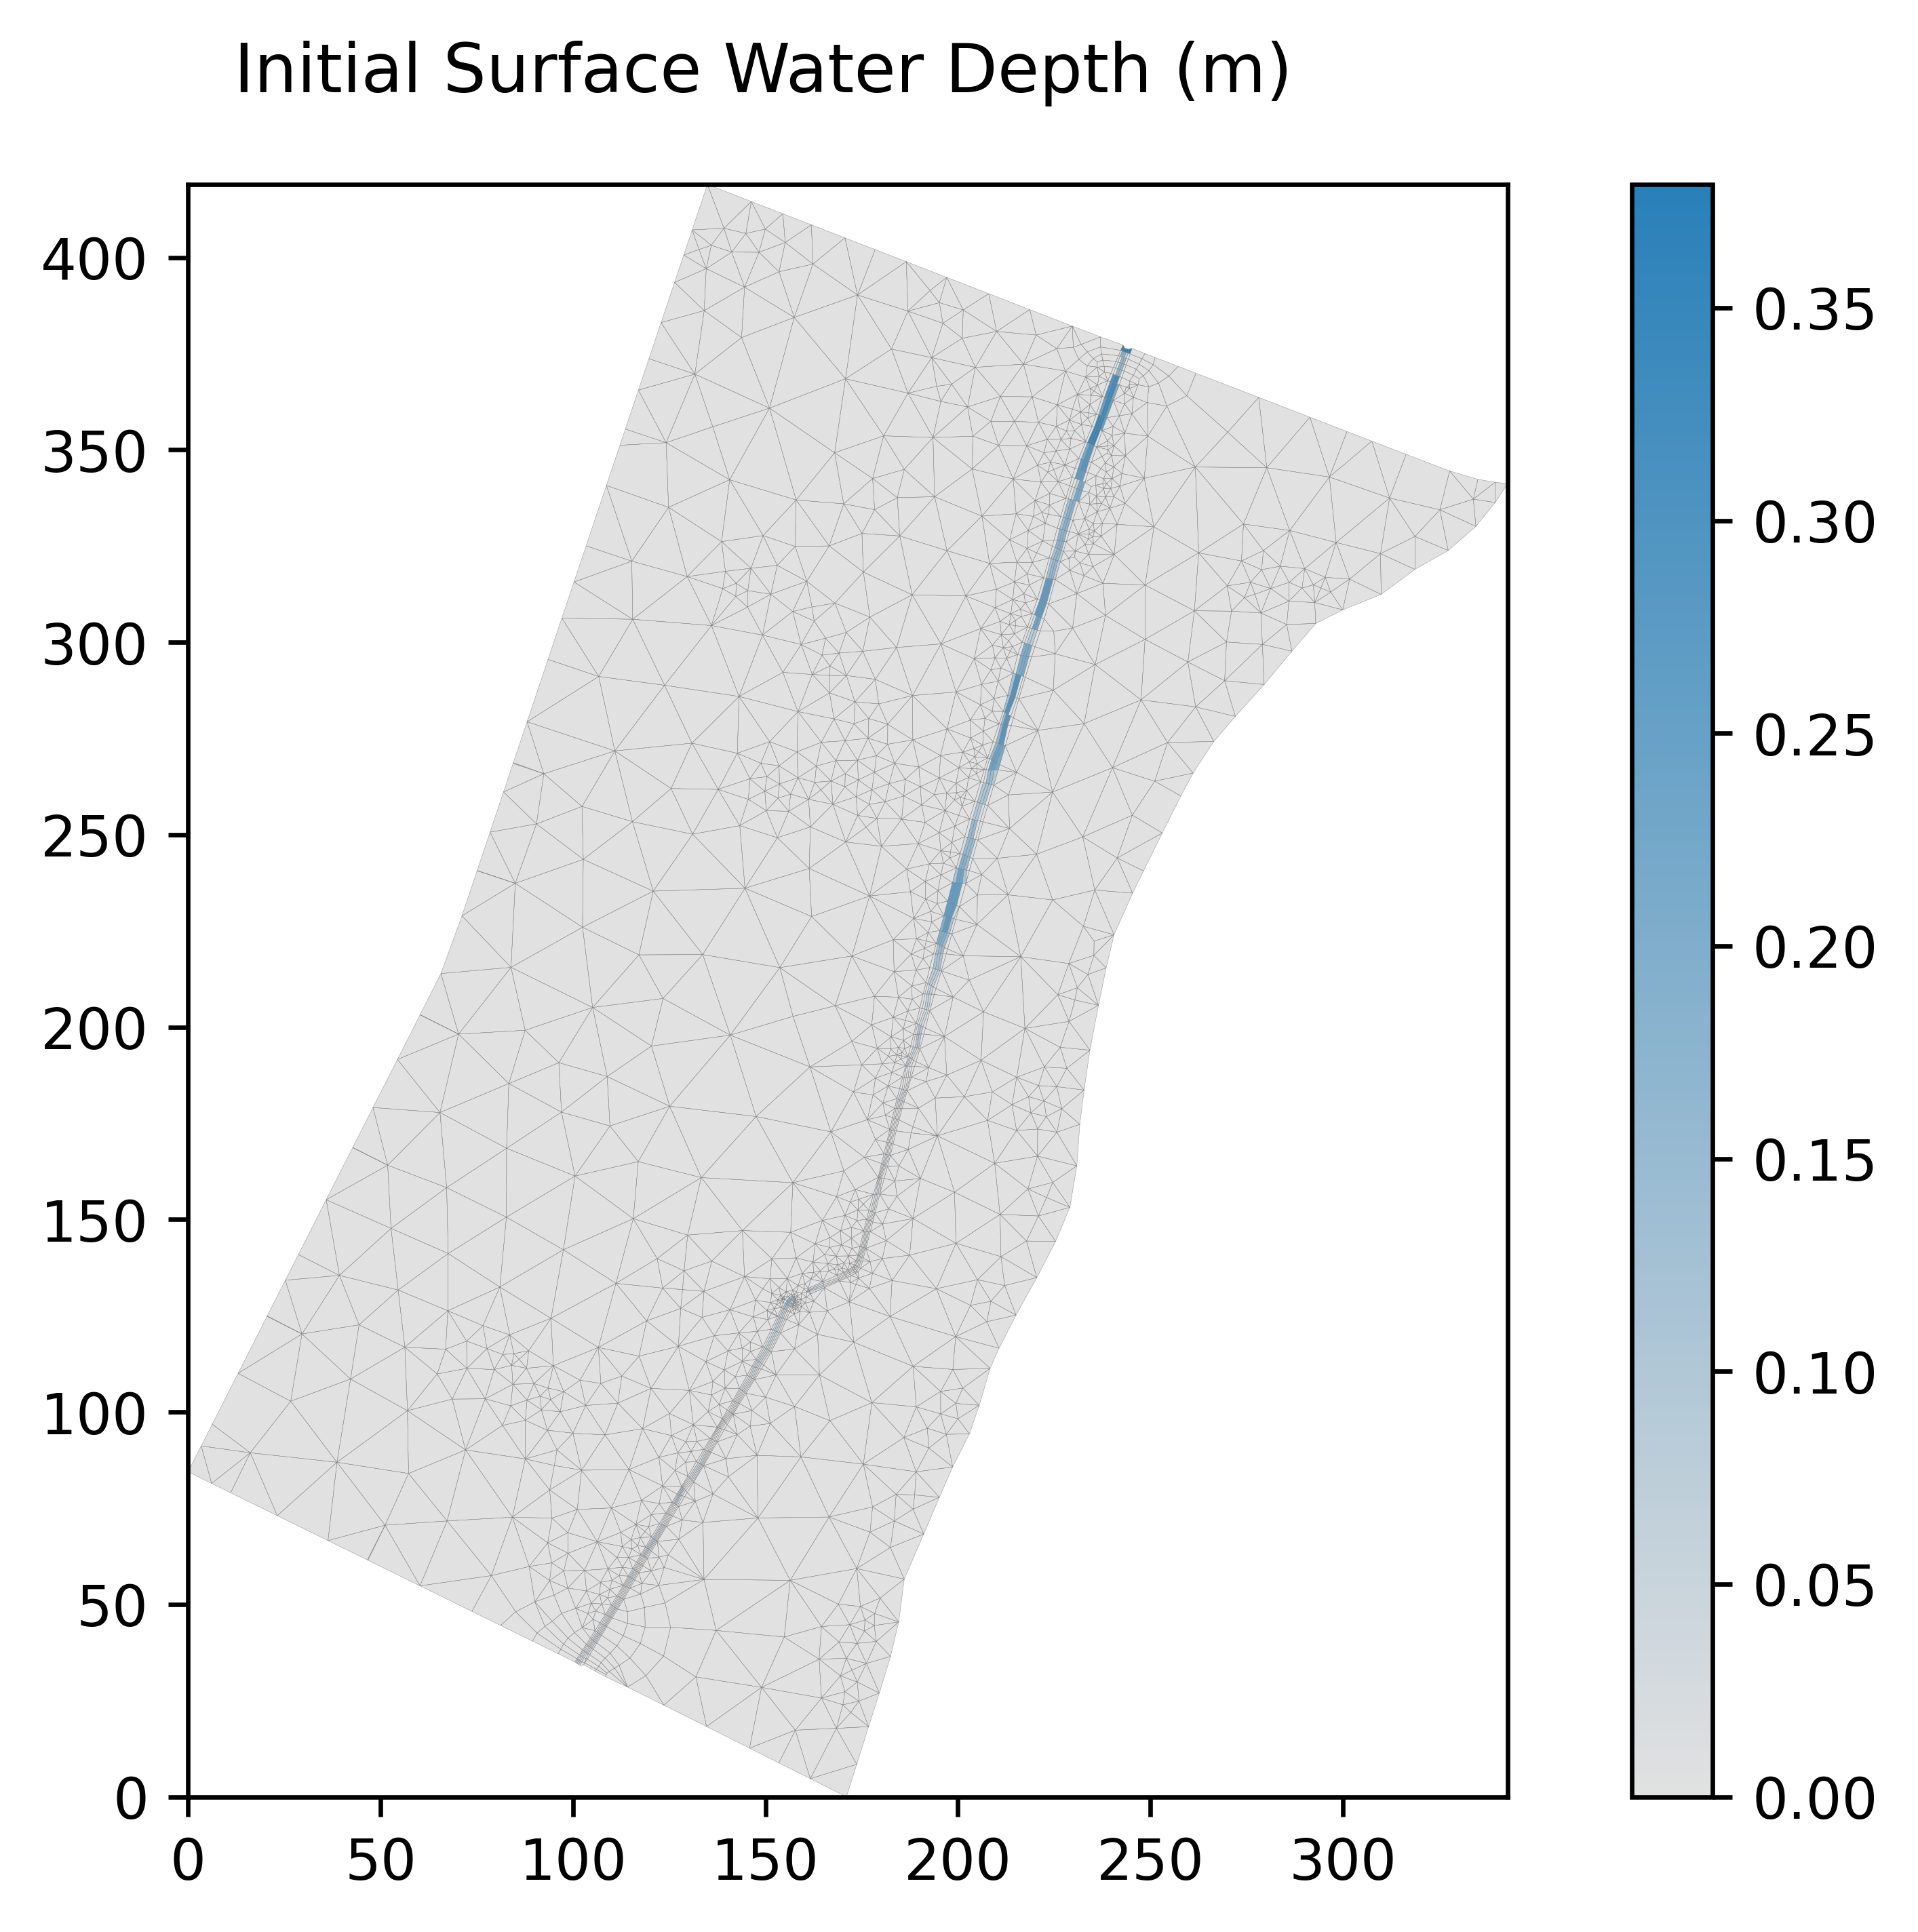
\includegraphics[scale=1]{PICTURES/models_ini/sws_ini.png}
    \caption{Initial Surface Water levels.}
    \label{fig:delft_iniWL}
\end{figure}


\section{Boundary Conditions}

\subsection{GWSWEX}
Grid elements that are bound by constant-head (CHD) boundary conditions in the GW model are flagged in the GWSWEX model so that the numerical scheme does not try to alter the GW heads, as observed by the illustration of the numerical scheme in Figure \ref{fig:GWSWEX_flow}.

\subsection{Modflow 6}
A constant head (CHD) boundary for the confined aquifer is set along the eastern boundary of the model grid as seen in Figure \ref{fig:grid_qgis}. The heads here are set to the surface level elevation based on speculation. \\
Along the stream, a CHD boundary is set in grid elements of the unconfined aquifer in locations that exhibit the presence of surface-water in the SW model at the end of the previous local simulation period. This boundary condition is thus dynamically updated every local simulation period with water levels read from the SW model.

\subsection{D-Flow FM}
A water level boundary condition is enforced along the northern-most grid elements in the stream, as seen by the elements marked by red in this area in Figure \ref{fig:grid_qgis}. The water levels for this enforcement is obtained from a water level observation at this location in the study area. Thus, with this enforcement, the initial water level in the SW model is as illustrated in Figure \ref{fig:delft_iniWL}.


\section{Observations}
Figure \ref{fig:obs_pts} shows the locations of GW observations located in the model domain. An SW observation is located as described in the previous section. However, since data from that observation is directly used to enforce a boundary condition in the SW model, it is of no relevance to compare model results to measured observations.

\begin{figure}[h!]
    \centering
    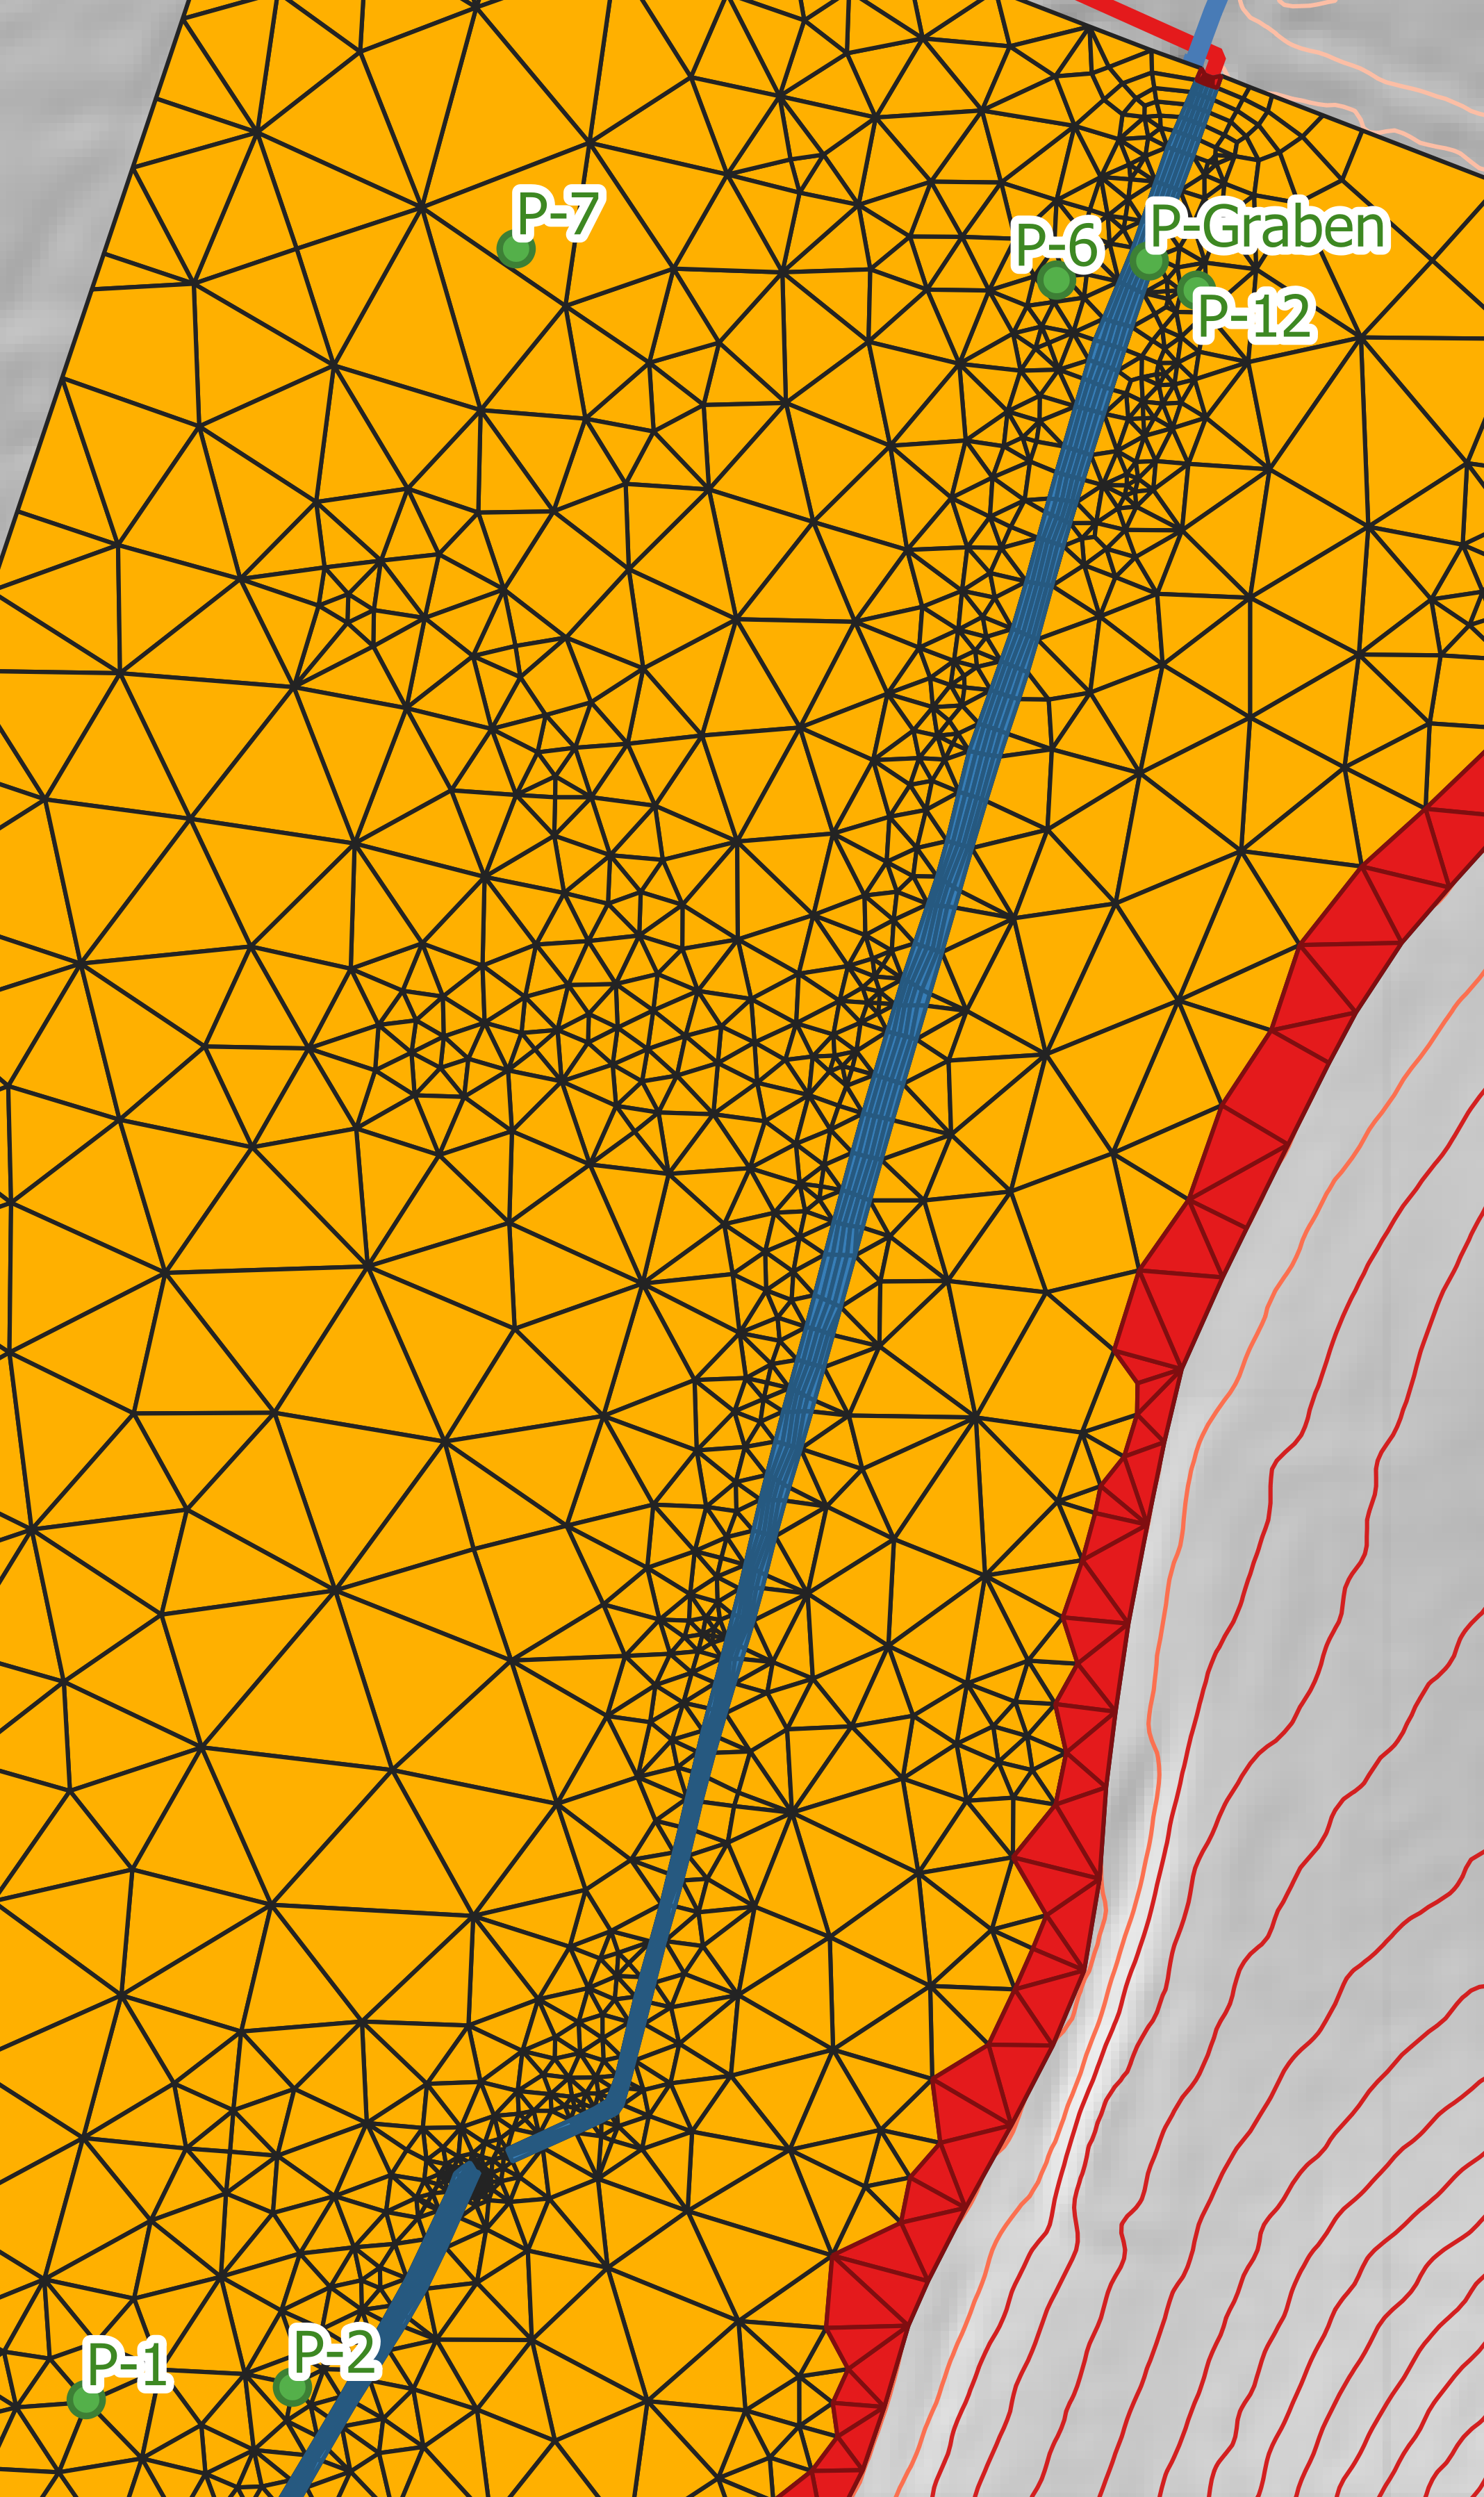
\includegraphics[height=\textheight]{PICTURES/models_ini/obs_pts.png}
    \caption{Locations of GW observation points.}
    \label{fig:obs_pts}
\end{figure}

\endinput